% !TEX root = ../thesis.tex

\chapter{Meranie kvantových obvodov}

Jediným spôsobom ako zistiť skutočný stav kvnatového obvodu je meraním.
Merať možno všetky bity súčasne ako aj jednotlivé kvantové bity samostatne.

\section{Princíp merania kvantových obvodov}

Kvantový bit môže existovať v nekonečnom množstve stavov. Meranie si môžme 
predstaviť ako prevod stavov kvantových bitov do stavu klasického digitálneho
systému \cite{Nie10}. Pre príklad môžeme reprezentovať kvantový stav 
\(\alpha\ket{0} + \beta\ket{1}\) pomocou nulového a excitovaného stavu atómu.
Skutočný kvantový počítač by tak mohol merať tieto stavy. Pri meraní by 
daný atóm skolaboval do jedného zo stavov \(\ket{0}\) alebo \(\ket{1}\).
Pre kolabovanie samozrejme rovnako platí to, že do jednotlivých stavov by
sa atóm dostal s pravdepodobnosťami \(|\alpha|^2\) respektíve \(|\beta|^2\).


Pri každom fyzikálnom meraní nastáva určitá nepresnosť merania. Takisto 
pri meraní môže dokonca nastať zničenie obvodu. To vyplíva z toho, že pri
skolabovanom kvantovom bite nastáva zmena fizykálnych vlastností daného bitu. 

\section{Fiktívne meranie}

Našim cieľom je navrhnúť pravdepodobnostný model, ktorý by umožnil merať
stavy kvantových obvodov aj bez kolabovania jednotlivých kvantových bitov.

\subsection{Experiment 1}
Navrhnime kvantový obvod s dvoma bitmi. Označme ich \(\ket{\psi_0}\) a 
\(\ket{\psi_1}\). V prvom kroku aplikujeme Hadamardovo hrado na bit 
\(\ket{\psi_0}\). Nasledovať budú dve \(CNOT\) hradlá, s opačnými kontrólnymi 
a cieľovými bitmi. V IBM QX je tento obvod reprezenovaný ako 
\begin{code}
qreg q[2];
creg c[2];

h q[0];
cx q[0],q[1];
cx q[1],q[0];
\end{code}
Jeho grafické zobrazenie je na obrázku \ref{expr1_circuit}, aj s označenými
časovými úsekmi, v ktorých bude meraný stav systému. 

\begin{figure} 
	\centering 
	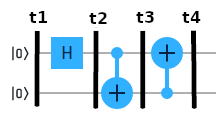
\includegraphics[width=.6\textwidth]{figures/expr1_circuit.png} 
	\caption{Obvod experimentu 1 s označenými časovými úsekmi meraní.}
    \label{expr1_circuit}
\end{figure}

\subsection*{Teoretická analýza}
Kvantové bity \(\ket{\psi_0}\) a \(\ket{\psi_2}\) sú definované ako 
\[\ket{\psi_0} = \alpha_0\ket{0} + \beta_0\ket{1}\]
\[\ket{\psi_1} = \alpha_1\ket{0} + \beta_1\ket{1}\]
, a teda je zrejmé, že v čase \(t_1\) pre celkový stav \(\ket{\psi}\) platí 
\[\ket{\psi} = \ket{\psi_0} \otimes \ket{\psi_1} = \alpha_0\alpha_1\ket{00} + \alpha_0\beta_1\ket{01} + \beta_0\alpha_1\ket{10} + \beta_0\beta_1\ket{11}\]

Z čoho jasne vyplíva, že systém nadobudne stav
    \begin{itemize}
        \item[] \(\ket{00}\) s pravdepodobnosťou \(|\alpha_0\alpha_1 |^2\)
        \item[] \(\ket{01}\) s pravdepodobnosťou \(| \alpha_0\beta_1 |^2\)
        \item[] \(\ket{10}\) s pravdepodobnosťou \(| \beta_0\alpha_1 |^2\)
        \item[] \(\ket{11}\) s pravdepodobnosťou \(| \beta_0\beta_1 |^2\) 
    \end{itemize}

Po prechode Hadamardovim hradlom, v čase \(t_2\) kvantové bity zmenia svoj stav
 na
\[\ket{\psi_0} = \frac{\alpha_0 + \beta_0}{\sqrt{2}}\ket{0} + \frac{\alpha_0 - \beta_0}{\sqrt{2}}\ket{1}\]
\[\ket{\psi_1} = \alpha_1\ket{0} + \beta_1\ket{1}\]

, a teda pre celkový stav \(\ket{\psi}\) bude platiť
\[\ket{\psi} = \frac{\alpha_0 + \beta_0}{\sqrt{2}}\alpha_1\ket{00} + \frac{\alpha_0 + \beta_0}{\sqrt{2}}\beta_1\ket{01} + \frac{\alpha_0 - \beta_0}{\sqrt{2}}\alpha_1\ket{10} + \frac{\alpha_0 - \beta_0}{\sqrt{2}}\beta_1\ket{11}\]

Kvantoý systém kolabuje v čase \(t_2\) do stavu
    \begin{itemize}
        \item[] \(\ket{00}\) s pravdepodobnosťou \(|\frac{\alpha_0 + \beta_0}{\sqrt{2}}\alpha_1|^2\)
        \item[] \(\ket{01}\) s pravdepodobnosťou \(|\frac{\alpha_0 + \beta_0}{\sqrt{2}}\beta_1|^2\)
        \item[] \(\ket{10}\) s pravdepodobnosťou \(|\frac{\alpha_0 - \beta_0}{\sqrt{2}}\alpha_1|^2\)
        \item[] \(\ket{11}\) s pravdepodobnosťou \(|\frac{\alpha_0 - \beta_0}{\sqrt{2}}\beta_1|^2\) 
    \end{itemize}

Zmena nastáva v čase \(t_3\), po prechode \(CNOT\) hradlom. Bit \(\ket{\psi_1}\)
bude preklopený len v prípade, že \(\ket{\psi_0}\) kolabuje do stavu 
\(\ket{1}\). A teda nastávajú dve možnosti. S pravdepodobnosťou 
\(|\frac{\alpha_0 + \beta_0}{\sqrt{2}}|^2\), ktorú označíme ako \(P^{t3}_1\) sa 
stavy kvantových bitov nezmenia
\[\ket{\psi_0} = \frac{\alpha_0 + \beta_0}{\sqrt{2}}\ket{0} + \frac{\alpha_0 - \beta_0}{\sqrt{2}}\ket{1}\]
\[\ket{\psi_1} = \alpha_1\ket{0} + \beta_1\ket{1}\]

Naopak, bit \(\ket{\psi_0}\) kolabuje do stavu \(\ket{1}\) s pravdepodobnosťou
\(|\frac{\alpha_0 - \beta_0}{\sqrt{2}}|^2\) (označme \(P^{t3}_{2}\)), a teda 
v tomto prípade nastáva zmena v kvantovom bite \(\ket{\psi_1}\)
\[\ket{\psi_1} = \beta_1\ket{0} + \alpha_1\ket{1}\]

Platí, že systém v čase \(t_3\) môže kolabovať do stavu
    \begin{itemize}
        \item[] \(\ket{00}\) s pravdepodobnosťou \((|\frac{\alpha_0 + \beta_0}{\sqrt{2}}\alpha_1|^2 \times P^{t3}_1) + (|\frac{\alpha_0 + \beta_0}{\sqrt{2}}\beta_1|^2 \times P^{t3}_{2})\)
        \item[] \(\ket{01}\) s pravdepodobnosťou \((|\frac{\alpha_0 + \beta_0}{\sqrt{2}}\beta_1|^2 \times P^{t3}_1 ) +(|\frac{\alpha_0 + \beta_0}{\sqrt{2}}\alpha_1|^2 \times P^{t3}_2)\)
        \item[] \(\ket{10}\) s pravdepodobnosťou \((|\frac{\alpha_0 - \beta_0}{\sqrt{2}}\alpha_1|^2 \times P^{t3}_1) +  (|\frac{\alpha_0 - \beta_0}{\sqrt{2}}\beta_1|^2 \times P^{t3}_2)\)
        \item[] \(\ket{11}\) s pravdepodobnosťou \((|\frac{\alpha_0 - \beta_0}{\sqrt{2}}\beta_1|^2 \times P^{t3}_1) +(|\frac{\alpha_0 - \beta_0}{\sqrt{2}}\alpha_1|^2 \times P^{t3}_2)\) 
    \end{itemize}


Poslendé meranie v tomto experimente je označené ako \(t_4\). Opäť nástáva
aktivácia \(CNOT\) hradla a teda podmienená zmena stavov kvantových bitov.
V každom prípade bit \(\ket{\psi_1}\) ostane nezmenený. No už teraz vychádzame 
z dvoch možností. Teda môžu nastať celkovo štyri pípady. V tabuľke 
\ref{expr1_t4_states} sú všetky možné zmeny stavov \(\ket{\psi_0}\) a
\(\ket{\psi_1}\).

\begin{table}
\centering
\begin{tabular}{|l|c|}
\hline
\textbf{Pravdepodobnosť} & \textbf{Stavy \(\ket{\psi_0}\) a \(\ket{\psi_1}\)} \\
\hline
\(P^{t4}_1 = |\frac{\alpha_0 + \beta_0}{\sqrt{2}}\alpha_1|^2\) & 
\(\ket{\psi_0} = \frac{\alpha_0 + \beta_0}{\sqrt{2}}\ket{0} + \frac{\alpha_0 - \beta_0}{\sqrt{2}}\ket{1}\) \\
& \(\ket{\psi_1} = \alpha_1\ket{0} + \beta_1\ket{1}\) \\
\hline

\(P^{t4}_2 = |\frac{\alpha_0 + \beta_0}{\sqrt{2}}\beta_1|^2\) & 
\(\ket{\psi_0} = \frac{\alpha_0 - \beta_0}{\sqrt{2}}\ket{0} + \frac{\alpha_0 + \beta_0}{\sqrt{2}}\ket{1}\) \\
& \(\ket{\psi_1} = \alpha_1\ket{0} + \beta_1\ket{1}\) \\
\hline

\(P^{t4}_3 = |\frac{\alpha_0 - \beta_0}{\sqrt{2}}\beta_1|^2\) & 
\(\ket{\psi_0} = \frac{\alpha_0 + \beta_0}{\sqrt{2}}\ket{0} + \frac{\alpha_0 - \beta_0}{\sqrt{2}}\ket{1}\) \\
& \(\ket{\psi_1} = \beta_1\ket{0} + \alpha_1\ket{1}\) \\
\hline

\(P^{t4}_4 = |\frac{\alpha_0 - \beta_0}{\sqrt{2}}\alpha_1|^2\) & 
\(\ket{\psi_0} = \frac{\alpha_0 - \beta_0}{\sqrt{2}}\ket{0} + \frac{\alpha_0 + \beta_0}{\sqrt{2}}\ket{1}\) \\
& \(\ket{\psi_1} = \beta_1\ket{0} + \alpha_1\ket{1}\) \\
\hline

\end{tabular}

\caption{\label{expr1_t4_states} Tabuľka stavov kvantových bitov a pravedpodobností
nastatia týchto stavov v čase \(t_4\) experimentu 1.}
\end{table}

Čiže celkový stav \(\ket{\psi}\) nadobudne stav
    \begin{itemize}
        \item[] \(\ket{00}\) s pravdepodobnosťou \\
\((|\frac{\alpha_0 + \beta_0}{\sqrt{2}}\alpha_1|^2 \times P^{t4}_1) + (|\frac{\alpha_0 - \beta_0}{\sqrt{2}}\alpha_1|^2 \times P^{t4}_2) + (|\frac{\alpha_0 + \beta_0}{\sqrt{2}}\beta_1|^2 \times P^{t4}_3) + (|\frac{\alpha_0 - \beta_0}{\sqrt{2}}\beta_1|^2 \times P^{t4}_4)\)

        \item[] \(\ket{01}\) s pravdepodobnosťou \\
 \((|\frac{\alpha_0 + \beta_0}{\sqrt{2}}\beta_1|^2 \times P^{t4}_1) + (|\frac{\alpha_0 - \beta_0}{\sqrt{2}}\beta_1|^2 \times P^{t4}_2) + (|\frac{\alpha_0 + \beta_0}{\sqrt{2}}\alpha_1|^2 \times P^{t4}_3) + (|\frac{\alpha_0 - \beta_0}{\sqrt{2}}\alpha_1|^2 \times P^{t4}_4)\)

        \item[] \(\ket{10}\) s pravdepodobnosťou \\ 
\((|\frac{\alpha_0 - \beta_0}{\sqrt{2}}\alpha_1|^2 \times P^{t4}_1) + (|\frac{\alpha_0 + \beta_0}{\sqrt{2}}\alpha_1|^2 \times P^{t4}_2) + (|\frac{\alpha_0 - \beta_0}{\sqrt{2}}\beta_1|^2 \times P^{t4}_3) + (|\frac{\alpha_0 + \beta_0}{\sqrt{2}}\beta_1|^2 \times P^{t4}_4)\)

        \item[] \(\ket{11}\) s pravdepodobnosťou \\
\((|\frac{\alpha_0 - \beta_0}{\sqrt{2}}\beta_1|^2 \times P^{t4}_1) + (|\frac{\alpha_0 + \beta_0}{\sqrt{2}}\beta_1|^2 \times P^{t4}_2) + (|\frac{\alpha_0 - \beta_0}{\sqrt{2}}\alpha_1|^2 \times P^{t4}_3) + (|\frac{\alpha_0 + \beta_0}{\sqrt{2}}\alpha_1|^2 \times P^{t4}_4)\)
    \end{itemize}

\subsection*{Výpočet pravdepodobností pomocou pravdepodobnostného modelu}
Pre použitie pravdepodobnostného modelu je nutné definovať obvod v jazyku 
Haskell. Vyjadrime jednotlivé hradlá a rozdeľme ich po vertikálnych leveloch.
\begin{code}
let l1 = Level [E, E] True
    l2 = Level [H, E] True
    l3 = Level [Cc, Ct] True
    l4 = Level [Ct, Cc] True
\end{code}
Pre meranie aj v čase \(t_1\), čiže ešte pred aktiváciou akéhokoľvek hradla,  
sme vložili jeden prázdny level navyše. Uložme tento obvod do spoločného listu
a definujme aj stromové štruktúry pre stavy a výsledky.
\begin{code}
c = [l1, l2, l3, l4]
st = StateTree 1 [q0, q0] []
rt = RT st []
\end{code}

Teraz už len spustime pravdepodobnostný model a uložme výsledky.
\begin{code}
let resultRT = processCircuit c rt
\end{code}

\begin{table}
\centering
\begin{tabular}{|c|}
\hline
1.0 \\ 
00 \\ 
\hline
\end{tabular}

\begin{tabular}{|c|c|}
\hline
0.5000000000000001 & 0.4999999999999999 \\ 
00 & 10 \\ 
\hline
\end{tabular}

\begin{tabular}{|c|c|c|c|}
\hline
0.25 & 0.2499999999999999 & 0.2500000000000001 & 0.25 \\ 
01 & 11 & 00 & 10 \\ 
\hline
\end{tabular}

\begin{tabular}{|c|c|c|c|c|c|}
\hline
0.25 & 0.2499999999999999 & 0.0 & 0.0 & 0.2500000000000001 & 0.25 \\ 
01 & 11 & 01 & 11 & 00 & 10 \\ 
\hline
\end{tabular}
\caption{\label{expr1_vystup} Výstup pravdepodobnostného modelu pre experiment 1
. Ohraničené riadky vymedzujú výsledky v jednotlivých časoch merania. Každá
bunka obsahuje pravdepodobnosť dosiahnutia stavu a daný stav systému.}
\end{table}

Pre vstupy kde na začiatku obvodu je \(\ket{\psi_0} = \ket{0}\) a zároveň
\(\ket{\psi_1} = \ket{0}\) nám model vypočítal výsledky, ktoré sú zaznamenané
v tabuľke \ref{expr1_vystup}. Každý ohraničený riadok predstavuje časový úsek.
Každá bunka potom obsahuje možný stav systému v daný časový úsek, kde horné
číslo je pravdepodobnosť dosiahnutia tohto stavu v rozmedzí \(0\) až \(1\) a 
spodná hodnota určuje daný stav v tvare \(\psi_0\psi_1\).

\subsection{Experiment 2}
\subsection{Experiment 3}
